%%%%%%%%%%%%%%%%%%%%%%%%%%%%%%%%%%%%%%%%%%%%%%%%%%%%%%%%%%%%%%%%%%%%%%%%%%%%%%%%
%2345678901234567890123456789012345678901234567890123456789012345678901234567890
%        1         2         3         4         5         6         7         8

% \documentclass[letterpaper, 10 pt, conference]{ieeeconf}  % Comment this line out if you need a4paper

\documentclass[a4paper, 10pt, conference]{ieeeconf}      % Use this line for a4 paper

\IEEEoverridecommandlockouts                              % This command is only needed if 
                                                          % you want to use the \thanks command

\overrideIEEEmargins                                      % Needed to meet printer requirements.

%In case you encounter the following error:
%Error 1010 The PDF file may be corrupt (unable to open PDF file) OR
%Error 1000 An error occurred while parsing a contents stream. Unable to analyze the PDF file.
%This is a known problem with pdfLaTeX conversion filter. The file cannot be opened with acrobat reader
%Please use one of the alternatives below to circumvent this error by uncommenting one or the other
%\pdfobjcompresslevel=0
%\pdfminorversion=4

% See the \addtolength command later in the file to balance the column lengths
% on the last page of the document

% The following packages can be found on http:\\www.ctan.org
\usepackage{graphics} % for pdf, bitmapped graphics files
\usepackage{epsfig} % for postscript graphics files
%\usepackage{mathptmx} % assumes new font selection scheme installed
%\usepackage{times} % assumes new font selection scheme installed
%\usepackage{amsmath} % assumes amsmath package installed
%\usepackage{amssymb}  % assumes amsmath package installed

\title{\LARGE \bf
Autonomous Vehicle Competition Project Report
}


\author{Bailin Lu$^{1}$ Chusheng Ku$^{2}$ Ryan Cheng$^{3}$ Xiaolan Cai$^{4}$% <-this % stops a space
\thanks{*This work was not supported by any organization}% <-this % stops a space
\thanks{$^{1}$Bailin Lu, Mechanical Engineering,
        University of Colorado Boulder,
        {\tt\small balu9739@colorado.edu}}%
\thanks{$^{2}$Chusheng Ku, Computer Science,
        University of Colorado Boulder,
        {\tt\small Chusheng.Ku@colorado.edu}}%
\thanks{$^{1}$Ryan Cheng, ,
        University of Colorado Boulder,
        {\tt\small rych6608@colorado.edu}}%
\thanks{$^{1}$Xiaolan Cai, Computer Science,
        University of Colorado Boulder,
        {\tt\small xiaolan.cai@colorado.edu}}%
}


\begin{document}

\maketitle
\thispagestyle{empty}
\pagestyle{empty}

%%%%%%%%%%%%%%%%%%%%%%%%%%%%%%%%%%%%%%%%%%%%%%%%%%%%%%%%%%%%%%%%%%%%%%%%%%%%%%%%
\begin{abstract}

This report will introduce the autonomous vehicle we design and build that can operate itself in an unknown closed course. The techniques we use in building this car learned from class CSCI 5302 Advanced Robotics and open source online. To complete the task of the class, we need to make the car do some challenge. Challenge we select are list as following:
\begin{itemize}
\item Visual-inertial SLAM
\item Power slide around turns
\item Stop at a stop sign
\item Report on human-robot interaction with autonomous vehicles.

\end{itemize}
In this report, we will present the platform, system and algorithm we use and why we use them.
Introduction

\end{abstract}


%%%%%%%%%%%%%%%%%%%%%%%%%%%%%%%%%%%%%%%%%%%%%%%%%%%%%%%%%%%%%%%%%%%%%%%%%%%%%%%%
\section{INTRODUCTION}
The development of ‘self-driving’ or ‘autonomous’ car technologies have advanced to very promising levels in recent years and could become Commercially available within a few years\cite{self-dctb}. More and more company are working on this project including Tesla, BMW, Honda, Ford and so on. Self-driving car technologies could increase on-road safety, make transformation more efficient. Our job is to build a robot can drive itself in an unknown environment. This project helps us learn the algorithm and principle of a self-driving car.

The sensor of our robot are oCam,IMU and two IR sensors. Although the sensors are much cheaper and simpler than the sensor use in self-driving cars. We still can learn the control method and mathematical model by working on the tasks.
Our whole system works on the Robot Operating System (ROS). ROS is a flexible framework for writing robot software. It has lots of tools, libraries, and conventions that aim to simplify the task of creating robot behavior across a wide variety of robotic platforms. In ROS, publisher will continually broadcast message to subscriber. Each sensor is a node that publish data like IMU (inertial measurement unit), IR (InfraRed) sensor and camera. Motor and servo motor are our subscriber. Order will be sent to motors to control the car can turn in corner, go straight in corridor or stop in front of stop sign.

As to the three challenge we finished. The first challenge is visual-inertial SLAM. SLAM (Simultaneous Localization And Mapping) has been a very active and almost ubiquitous problem in the field of mobile and autonomous robotics for over two decades\cite{roslam}.

It is the computational problem of updating a map of an unknown environment while simultaneously keeping track of agent’s location within it. Robot can locate itself by going in unknown environment repeated and scan terrain feature like pillar, wall, corner. The main algorithm is extended Kalman filter which is the nonlinear version of the Kalman filter. SLAM will always use several different types of sensors, and the powers and limits of various sensor types have been a major driver of new algorithms\cite{csvslam}. We combine 1042 PhidgetSpatial IMU with our oCam as our sensor. In the following section we will discuss visual-inertial SLAM in detail. Second challenge is stop at a stop sign. We use deep learning package train the camera then test it with printed stop on A4 paper. When we get high enough accuracy, we install the whole system in ROS and run with robot so that the robot can recognize the stop sign and stop immediately. Third challenge is power slide around turns. The basic idea is that by adjusting the PD parameter of the control system and speed of the car to make the robot drift. Last challenge is report about human-robot interaction with autonomous vehicles. You can read it in appendix.

\section{Visual-inertial SLAM}
Chusheng

\section{Robot Operating System}

\subsection{State Machine}

Ryan

\section{Stop at a stop sign}
One of the key aspects in building a fully autonomous self-driving car is to be able to track and detect objects around the vehicle. The challenge to stop at a stop sign gives us 

There are several approaches to detect a stop sign with the camera, such as pattern recognition, image classification or even simpler way as shape detector to detect an octagon shape with the OpenCV FindContours and ApproPolyDP method to approximate contours in an image. We choose to use deep learning method to accomplish this task since we have been taught in class and this would be good learning opportunity for us. 

We firstly tried several famous off-the-shelf pre-trained object detection models, such as Google's Mobilenet Object Detection API, and Darknet Tiny Yolo. Both models are trained on COCO dataset which has 80 real-world object categories including stop sign and sports ball and both are light weight deep neural network. 

After deploying and conducting experiments on Odroid platform, we found Mobilenet Object Detection is running too slow 

We choose to implement and train a customized convolution neural network image classifier to classify images with a stop sign.

\begin{figure}
    \centering
    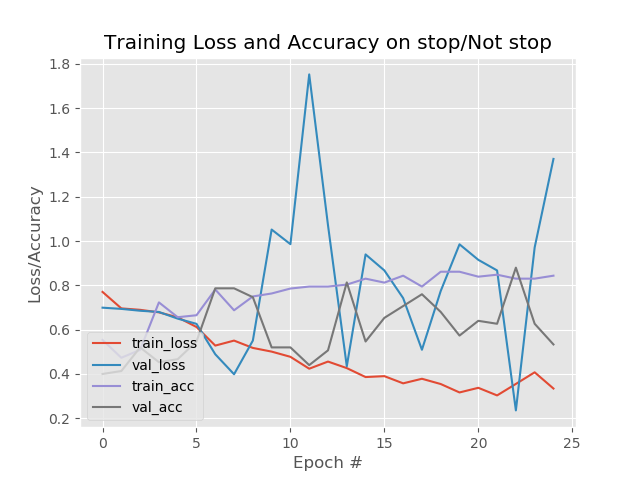
\includegraphics[width=8cm]{model_training.png}
    \caption{training loss and accuracy}
    \label{fig:model_training}
\end{figure}



\section{Electrical Part}

\subsection{ODROID XU-4}
ODROID-XU4 board is a powerful, energy-efficient hardware made by Samsung. We choose this board because it offers open source support, the board can run various flavors of Linux, including Ubuntu 16.04 and Android 4.4 KitKat and 7.1 Nougat. Ubuntu 16.04 is the system we use. ROS can run in Ubuntu 16.04 pretty good. So ODROID have good compatibility to our system. Also, it has 2 USB 3.0 Host and 1 USB 2.0 Host can meet the requirements because our camera, IMU and Polulu all need USB interface. 

It can boot from a MicroSD card or an eMMC module is convenient to use. Our project need to work on Linux system with ROS and need to complete many tasks. Enough storage is important to us. ODROID-XU4 have 2 Gbyte DDR3 RAM is big enough for us to do all the challenges.

\subsection{oCam 1MGN-U}

\subsection{IMU}
IMU have 3-axis compass, 3-axis gyroscope and 3-axis accelerometer. We combine IMU with oCam to do the visual-inertial SLAM. IMU was binding with camera so that we can confuse space data with camera image.
At first, the IMU need to be calibrated in order to get useful accuracy compass number. We can calculate magnetic field value of your place on internet. Then put the magnetic field value into program that Phidget designed for us to do the calibration. With IMU connect to the computer and rotate the compass around such that red dots (In Fig.?) being generated on the screen outline as much of a full sphere as possible. Then you can get parameter with calibrated data in it.

\begin{figure}
    \centering
    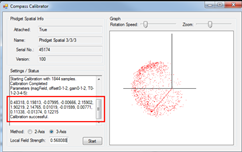
\includegraphics{IMU.png}
    \caption{IMU Calibration}
    \label{imu cali}
\end{figure}

\subsection{IR Sensor}
Our car should drive safely in corridor. IR sensor can help us not hitting on the wall. We set two sensors in front of our robot. One facing slightly to the left the other one facing slightly to the right. By computing the difference distance to left and right wall, we can set the plant as zero, the car will keep running in the middle of the corridor. When the robot getting to the corner, the difference will immediately change, we set the threshold as 200cm which means distance to left minus to the right is bigger than 200 or less than -200 means the car is in the corner. Then the robot will change to turning mode.

The IR sensor we use is GP2Y0A710K0F. It can measure distance between 100 to 550cm. Analog output type. One problem is that the sensor’s output is not linear. Distance measurement characteristics is shown in Fig.\ref{ir fig} We test the output depends on the distance and separate distance into three segments. Each segment has corresponding slope. In this way, we can get more accuracy data. As you can see the distance it can measure is more than 1 meter. When the distance is less than 1 meter, the data confuse controller because it is same as data more than 1 meter.
\begin{figure}
    \centering
    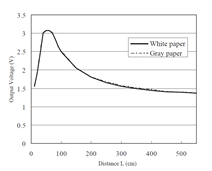
\includegraphics{IR.png}
    \caption{IR sensor distance measurement characteristics}
    \label{ir fig}
\end{figure}

\subsection{Polulu}
The Mini Maestro can direct connect to ODROID by USB. It has 18 channels. Each channel can be used as general-purpose digital outputs, Analog or digital inputs (channels 0-11 can be analog inputs; channel 12+ can be digital inputs). Polulu connect to Servo and ESC(electronic speed control) use output fuction. It get input signal from IR sensor then transfer the data to ODROID through USB.

\subsection{Voltage Divider}
The battery we use are two 7.2V 6 cell Ni-MH. The ODROINO, polulu and IR sensor all need 5V power. Drok voltage regulator can regulate voltage from 3~40V to 1.23~37V. We set the output to 5V power for our robot. The Output current can be up to 3A. XU4 board requires a 5V/4A DC power source which have more electric current than voltage divider can produce. When the battery is full charged, XU4 can work normally. But this can not last long. With the power loss, XU4 may shut down itself.

\section{Mechanical Part}

\subsection{Bumper}
We made bumper to protect our car from hitting the wall. We need to do racing of running the robot in the circle within 30s. The robot runs around 5m/s in the corridor. It is hard for us to keep up with car and catch it before it run into the wall. With a bumper in front of the car can absorb the energy of hitting and protect the electronic device. IMU and IR sensor are easily damaged. We have broken one of our IR when testing the car in the corner. The bumper can save lots of work repair the robot. I use acrylic board with foam tube together build the bumper show in Fig.\ref{bumper} The foam tube was fixed on the acrylic board by blue tape. We drill holes on the car so that we can use screw install the bumper on the car.
\begin{figure}[htp]
    \centering
    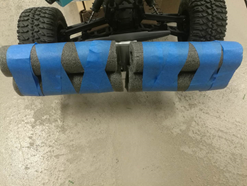
\includegraphics{bumper.png}
    \caption{Bumper}
    \label{bumper}
\end{figure}

\subsection{Platform}
All of our electric board except ESC are putting on the acrylic board cut by laser. We reserve some big holes at front and back of our robot so we can make the wire connect to ODROID can go downside of our platform and go up again near the XU4. This can make our robot looks concise.
\begin{figure}[htp]
    \centering
    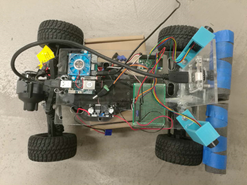
\includegraphics{platform.png}
    \caption{Platform}
    \label{platform}
\end{figure}

\subsection{IR stand}
At beginning of our project. We use IR stand shown in figure.? But we found that the position of screw hole at side of stand is not stable. It will turn a little bit when the robot hits the wall. Then we drop this plan and made a new one with screw hole at back of stand shown in Fig.\ref{io fig}. The new stand is much more stable than the old design. We use 3D printing to print out the stand with PLA.
\subsection{Camera stand}

The camera stand is more complex than the IR stand. Because the camera is more sensitive than IR. Good quality of image is important for us to get better result with visual SLAM. If the stand is too high, it will have more violent shaking at top. If the stand is too low, the camera will get less features from the image because nearly half of the image is ground. The color of ground doesn’t change too much. Also, there is less corner and line on the ground. We set the height as 16cm so that we can get good image features without too much shaking. To decrease the shaking, we add rib to fix the stand. We use hot glue combine rib and stand with our platform.
\begin{figure}[htp]
    \centering
    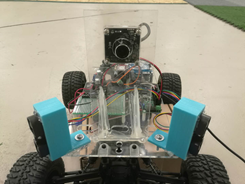
\includegraphics{Stand.png}
    \caption{IR and oCam stand}
    \label{io fig}
\end{figure}


\section{Control}

Bailin  Ryan

The final control configuration utilized two PID controllers running in parallel with a state machine to dynamically switch which control effort to publish to the servo controller.


\section{What We Learned}

Together

\section{Problems we met & how We fix them}

Together
\subsection{3D printing}
The most commonly used types of personal 3D printing are ABS and PLA. We build two IR sensor and Camera holder with PLA. Because PLA have less shrink than ABS. When ABS cools after printing it shrinks approximately 8\%. PLA shrinks approximately 2\%. It is not as much as ABS but big enough have influence on our IR stand. We first drawing the stand with Solidworks use parameter exactly same as IR sensor. After we print out the stand we found that we can not put IR sensor into it. Then we resize the stand and print it again get the one can fit IR sensor in it. Counting on the shrinking in the design part can improve the success rate of 3D printing and waste less material and time.
\section{Code}

Together

\section{CONCLUSIONS}

Together

%%%%%%%%%%%%%%%%%%%%%%%%%%%%%%%%%%%%%%%%%%%%%%%%%%%%%%%%%%%%%%%%%%%%%%%%%%%%%%%
% Following code shows how to insert figure and table. I left them here just in case you need it.

\begin{table}[h]
\caption{An Example of a Table}
\label{table_example}
\begin{center}
\begin{tabular}{|c||c|}
\hline
One & Two\\
\hline
Three & Four\\
\hline
\end{tabular}
\end{center}
\end{table}


   \begin{figure}[thpb]
      \centering
      \framebox{\parbox{3in}{We suggest that you use a text box to insert a graphic (which is ideally a 300 dpi TIFF or EPS file, with all fonts embedded) because, in an document, this method is somewhat more stable than directly inserting a picture.
}}
      %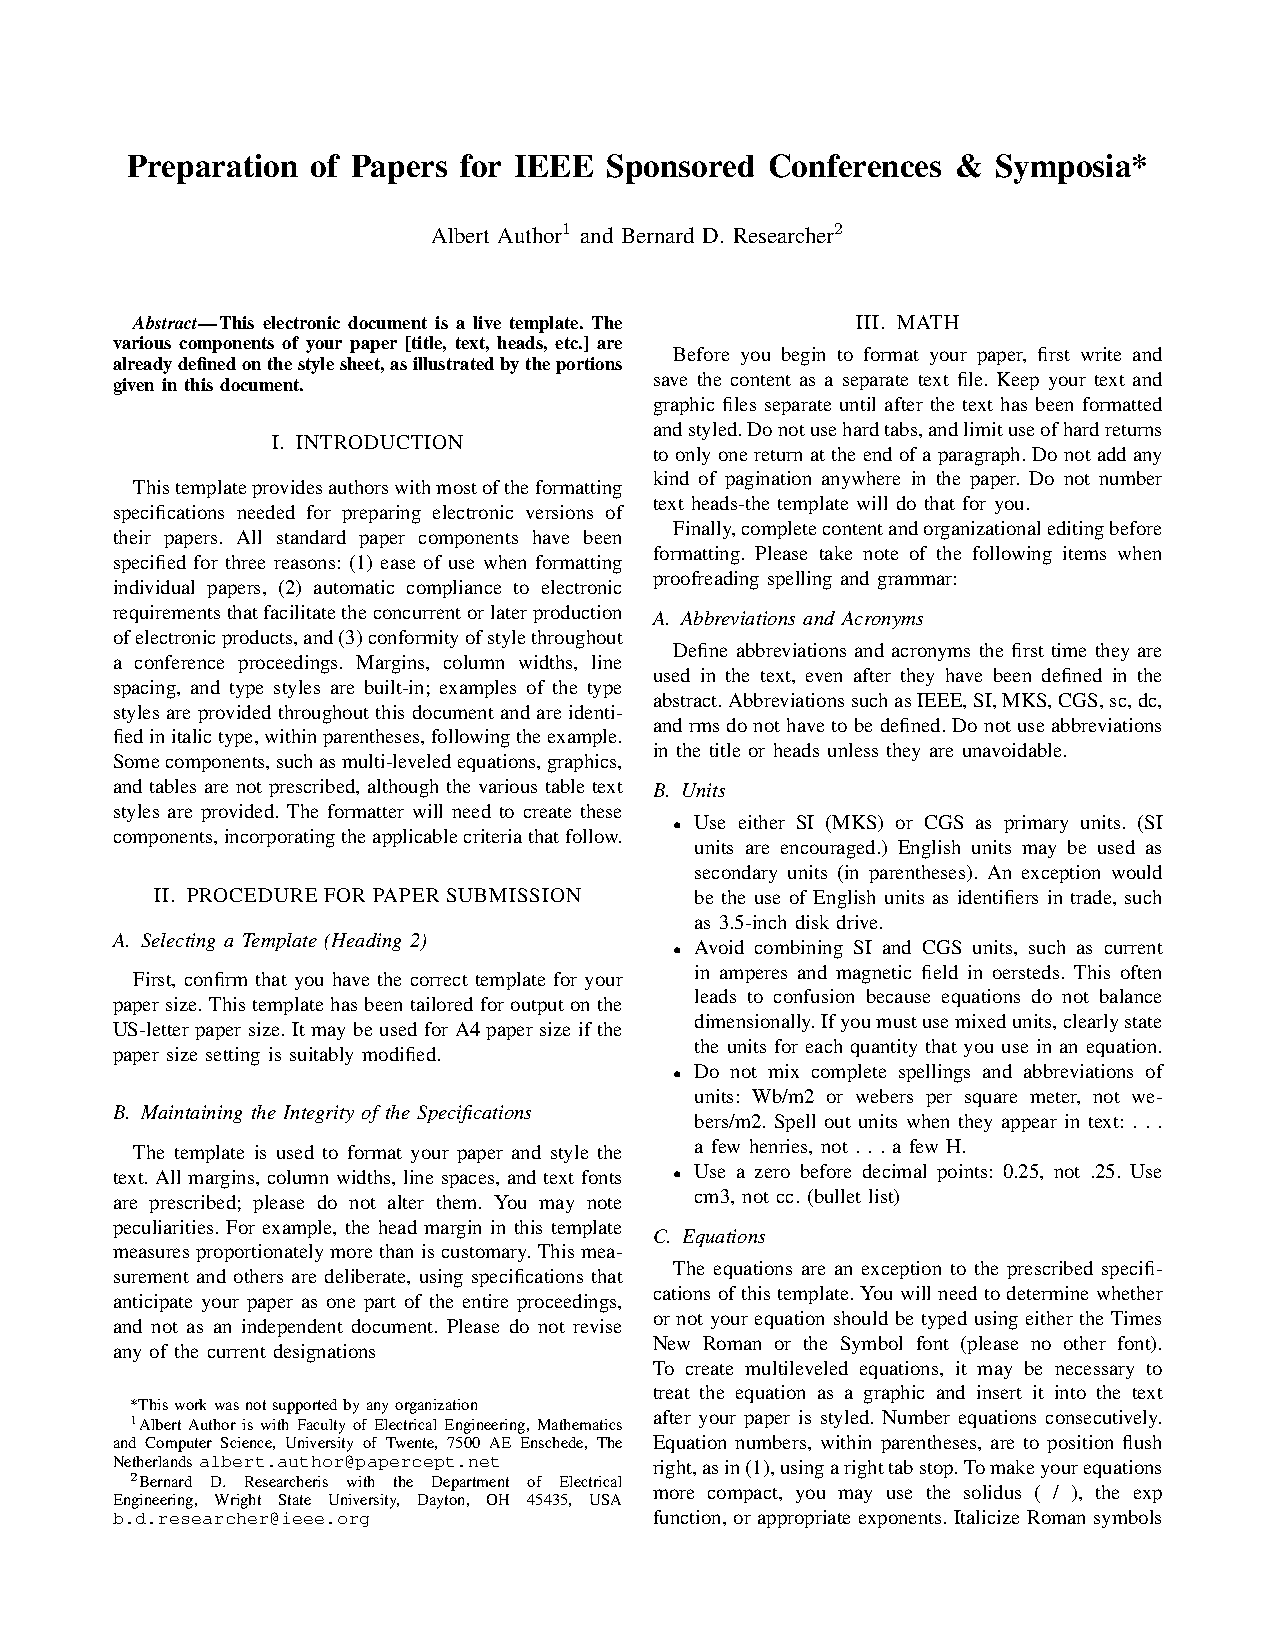
\includegraphics[scale=1.0]{Adv robot/root.pdf}
      \caption{Inductance of oscillation winding on amorphous
       magnetic core versus DC bias magnetic field}
      \label{figurelabel}
   \end{figure}
   
%%%%%%%%%%%%%%%%%%%%%%%%%%%%%%%%%%%%%%%%%%%%%%%%%%%%%%%%%%%%%%%%%%%%%%%%%%%%%%

\addtolength{\textheight}{-12cm}   % This command serves to balance the column lengths
                                  % on the last page of the document manually. It shortens
                                  % the textheight of the last page by a suitable amount.
                                  % This command does not take effect until the next page
                                  % so it should come on the page before the last. Make
                                  % sure that you do not shorten the textheight too much.

%%%%%%%%%%%%%%%%%%%%%%%%%%%%%%%%%%%%%%%%%%%%%%%%%%%%%%%%%%%%%%%%%%%%%%%%%%%%%%%%



%%%%%%%%%%%%%%%%%%%%%%%%%%%%%%%%%%%%%%%%%%%%%%%%%%%%%%%%%%%%%%%%%%%%%%%%%%%%%%%%



%%%%%%%%%%%%%%%%%%%%%%%%%%%%%%%%%%%%%%%%%%%%%%%%%%%%%%%%%%%%%%%%%%%%%%%%%%%%%%%%
\section*{APPENDIX}
\title{\LARGE \bf
Human-robot interaction with autonomous vehicles}




\begin{thebibliography}{99}

\bibitem{self-dctb}Miller, John (19 August 2014). "Self-Driving Car Technology's Benefits, Potential Risks, and Solutions". theenergycollective.com. Retrieved 4 June 2015.

\bibitem{roslam} Sünderhauf, Niko. Robust optimization for simultaneous localization and mapping. Diss. Technischen Universitat Chemnitz, 2012.

\bibitem{csvslam} Magnabosco, M., Breckon, T.P. (February 2013). "Cross-Spectral Visual Simultaneous Localization And Mapping (SLAM) with Sensor Handover" (PDF). Robotics and Autonomous Systems. 63 (2): 195–208. doi:10.1016/j.robot.2012.09.023. Retrieved 5 November 2013.

\bibitem{mobilenet} Andrew G. Howard ,Menglong Zhu ,Bo Chen, Dmitry Kalenichenko, Weijun Wang, Tobias Weyand, Marco Andreetto, Hartwig Adam. "MobileNets: Efficient Convolutional Neural Networks for Mobile Vision Applications". CoRR: abs/1704.04861.2017

\bibitem{yolo}Joseph Redmon,Santosh Kumar Divvala,Ross B. Girshick,Ali Farhadi. "You Only Look Once: Unified, Real-Time Object Detection". CoRR:abs/1506.02640. 2015

\bibitem{darknet}J. Redmon. Darknet: Open source neural networks in c. http://pjreddie.com/darknet/, 2013–2016





\end{thebibliography}

\end{document}
